\begin{figure}[ht]

\centering

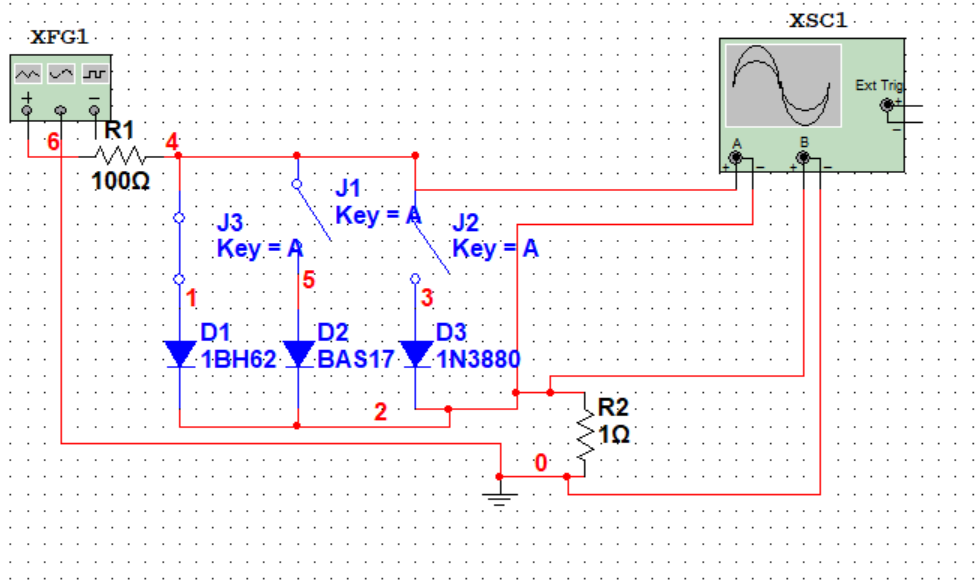
\includegraphics[width=0.6\linewidth]{Діод1Схема.png}

\caption{Схема}

\label{Diod1Shema}

\end{figure}

\begin{figure}[ht]

\centering

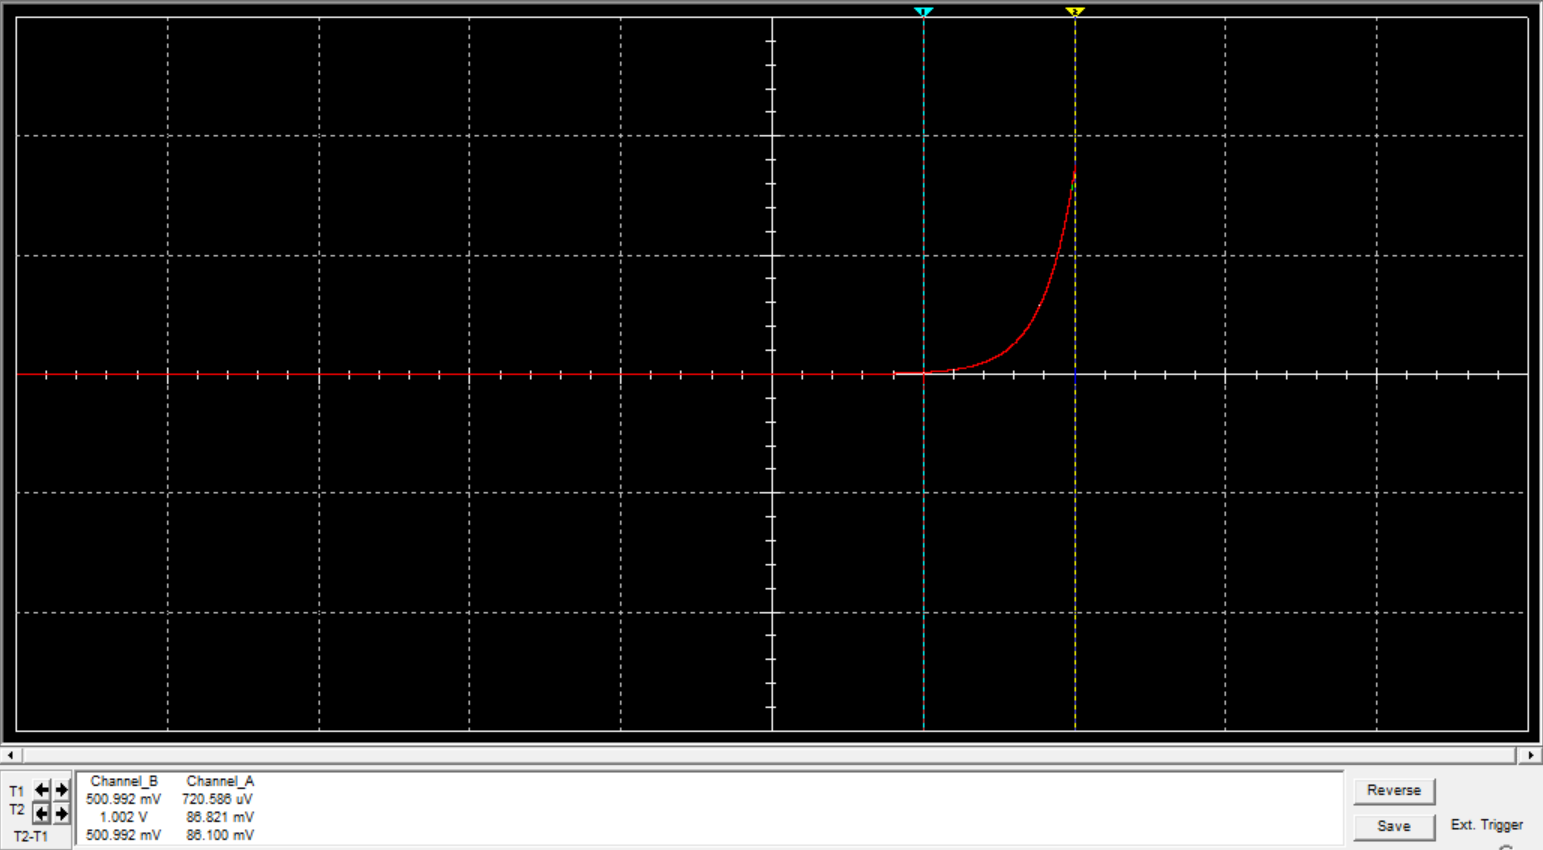
\includegraphics[width=0.75\linewidth]{Діод1Осцилограф.png}

\caption{Результати вимірів}

\label{Diod1Osc}

\end{figure}

\begin{figure}[ht]

\centering

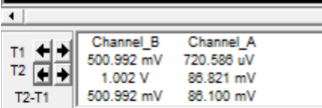
\includegraphics[width=0.3\linewidth]{Діод1Рез.png}

\caption{Результати вимірів}

\label{Diod1Rez}

\end{figure}

Оскільки канал А виводить напругу на резисторі опором $1  \Omega $, можемо вважати, що отримані значення - сила струму у колі.
